\section{Experiments}
\label{sec:experiments}

% \begin{description}
% 	\item [RNN] 10, 25, 50, 75, and 100 gated recurrent units.
% 	\item [Training] 200 epochs.
% 	\item [Learning curves] cost functions, accuracies, and some metric for weights.
% 	\item[Activations] of GRUs for tunes.
% 	\item[Evaluation] on test set as a table.
% 	\item [Reconstructions] of test examples.
% \end{description}

The experiments were run for the normal RNN model using only original input and the extended RNN model using the previous prediction step output as input. 



\subsection{Regularization} % (fold)
\label{sub:regularization}

Dropout of 20\% or 50\% was applied right before the GRU layer in the input network. By dropping out notes along the melodies, a lossy noise and therefore a completion task is introduced to the models, so during training the next-step prediction will rely more on the previous GRU activations $\vec{h}\idx{t-1}$ and the horizontal connections will be enhanced to make up for the missing input. The stronger horizontal connections will hopefully combine some more general musical rules and therefore reduce overfitting. 

An $L_2$-regularization term is also added to the total cost during training for reducing overfitting.
% subsection regularization (end)


\subsection{Evaluation}

The performance measures are the prediction accuracy and the two categorical cross entropy measures over pitch and duration classes are recorded for each epoch and seen in the learning curves.

Other measures used for model investigation are the mean, frobenius norm and positive value fractions over both the horizontal weights (hidden to hidden state) and vertical weights (input to hidden state), where the trend in the overall magnitude and sign of the weights are expected to be seen. \\ \\


The two models with and without dropout and/or regularization are tested for 10, 25, 50, 75, and 100 gated recurrent units, so scaling of performance can be investigated and the effect of the regularization methods compared. The scaling of performance with the number of GRU are clearly seen, but not shown here, so 100 GRU are used as a standard and for these regularization methods and model architectures can be compared in Table \ref{tab:test_eval}.

All models are trained for 200 epochs, as a clear convergence in the learning curves in Figure \ref{fig:learning_curves} and \ref{fig:learning_curves_regularized} were seen after 150 epochs of training. \\ \\

\subsection{Reconstructions}

After training, the models were evaluated on 2 test songs, handpicked out of the unseen test set. The notes in the original melody (input) are highlighted by colors corresponding to the GRU activations, so patterns, like scale and rhythmical motifs, leading to higher activation can be localized and the functionality of the GRU identified.

To investigate the distribution of the pitch and duration classes, the frequencies of each class in the original data are represented in a histogram in Figure~\ref{fig:histogram}

All reconstructions can be translated back to the \texttt{music21} format, written to a midi file, played, written as a musical score and compared against the original melody.

\begin{table*}
    \centering
    \caption{
        The test evalutation measures.
    }
    \label{tab:test_eval}
    % \setlength{\tabcolsep}{1em}
    \sisetup{
        table-number-alignment = center
    }
    \begin{tabular}{
            l@{}
            S[table-format = 1.0]
            S[table-format = 0.2]
            S[table-format = 1.0]
            S[table-format = 1.3]
            S[table-format = 1.3]
            S[table-format = 2.2]
            S[table-format = 2.2]
        }
        \toprule
        & {Model} 
        & {$p\idx{dropout}$}
        & {$\alpha_2$}
        & {$L\idx{pitch}$}
        & {$L\idx{duration}$}
        & {$A\idx{pitch}$(\%)}
        & {$A\idx{duration}$(\%)} \\
        \midrule
        \input{../data/eval_table}
        \bottomrule
    \end{tabular}
\end{table*}

\begin{figure*}
    \centering
	\hspace*{\fill}
    \subbottom[\label{fig:learning_curves:type1}]{
        \includegraphics[width = .45\linewidth]{Normal_GRU_Network_gru_100_bs_10_e_200_acc}
    }
    \hfill
    \subbottom[\label{fig:learning_curves:type2}]{
        \includegraphics[width = .45\linewidth]{GRU_using_deterministic_previous_output_gru_100_bs_10_e_200_acc}
    }
	\hspace*{\fill}
    \caption{Learning curves over next-step prediction accuracies for \subcaptionref{fig:learning_curves:type1} model type 1 and \subcaptionref{fig:learning_curves:type2} model type 2 without any regularization. The models are evaluated on both training (solid lines) and validation sets (dashed lines) and for pitch (turquoise) and duration classes (orange).)
    }
    \label{fig:learning_curves}
\end{figure*}

\begin{figure*}
    \centering
	\hspace*{\fill}
    \subbottom[\label{fig:learning_curves_regularized:type1}]{
        \includegraphics[width = .45\linewidth]{GRU_using_deterministic_previous_output_with_50p_dropout_gru_100_bs_10_e_200_acc.pdf}
    }
    \hfill
    \subbottom[\label{fig:learning_curves_regularized:type2}]{
        \includegraphics[width = .45\linewidth]{Normal_GRU_Network_with_50p_dropout_gru_100_bs_10_e_200_acc}
    }
	\hspace*{\fill}
    \caption{Learning curves over next-step prediction accuracies for \subcaptionref{fig:learning_curves_regularized:type1} model type 1 and \subcaptionref{fig:learning_curves_regularized:type2} model type 2, both with $50\%$ dropout. The models are evaluated on both training (solid lines) and validation sets (dashed lines) and for pitch (turquoise) and duration classes (orange).
    }
    \label{fig:learning_curves_regularized}
\end{figure*}


\begin{figure*}
    \centering
    \setkeys{Gin}{height=.25\textheight}
	\hspace*{\fill}
    \subbottom[\label{fig:histogram_orig:pitch}]{
        \includegraphics{orig_pitch_freq_barplot}
    }
    \hfill
    \subbottom[\label{fig:histogram_orig:duration}]{
        \includegraphics{orig_duration_freq_barplot}
    }
	\hspace*{\fill}
    \caption{Histograms showing statistical frequency of pitch \subcaptionref{fig:histogram_orig:pitch} and duration \subcaptionref{fig:histogram_orig:duration} classes.)
    }
    \label{fig:histogram}
\end{figure*}

\begin{figure*}
    \centering
    \setkeys{Gin}{height=.25\textheight}
	\hspace*{\fill}
    \subbottom[\label{fig:histogram_models:pitch}]{
        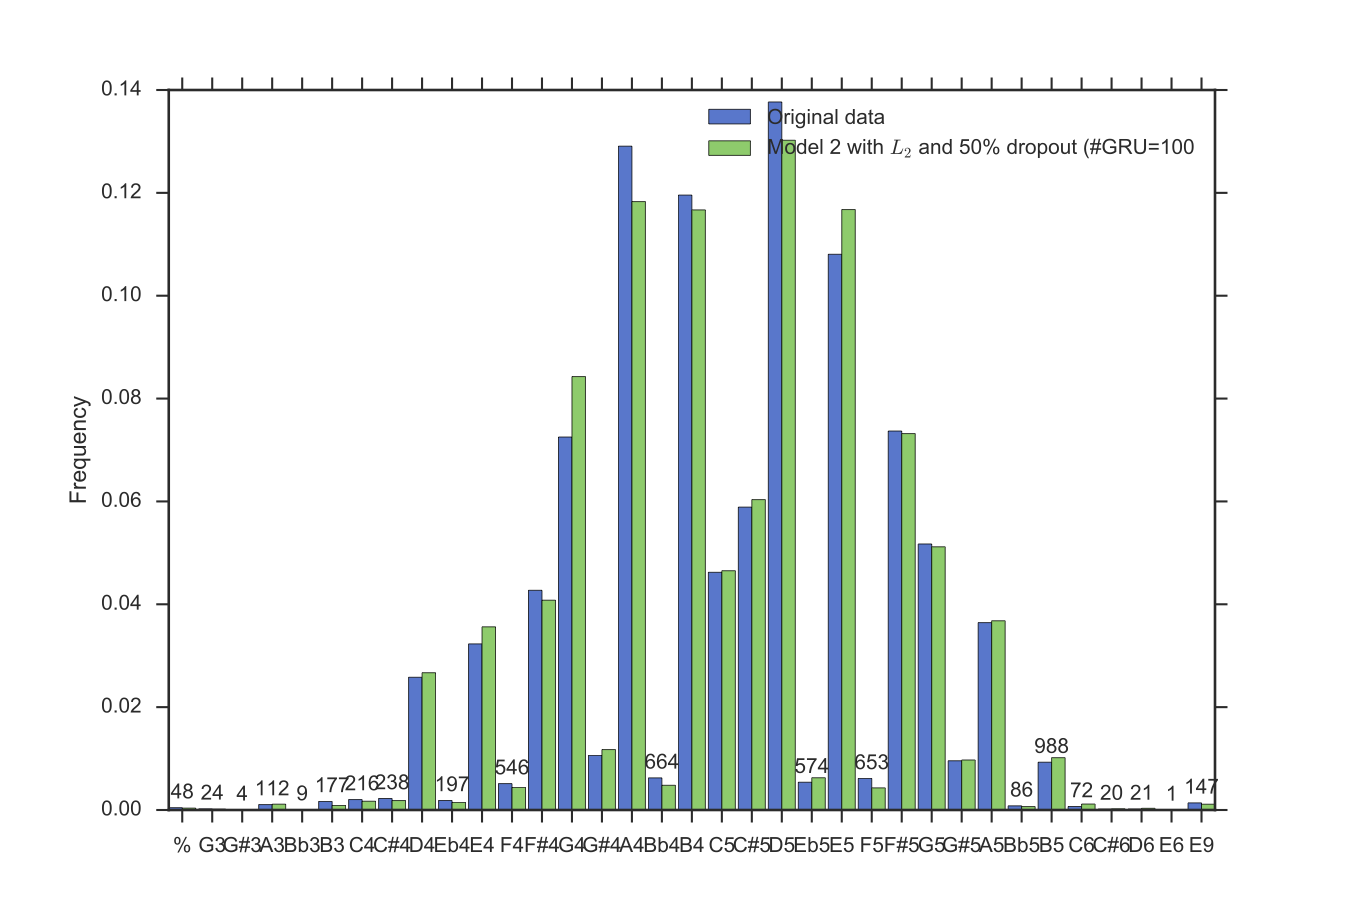
\includegraphics{models_pitch_freq_barplot}
    }
    \hfill
    \subbottom[\label{fig:histogram_models:duration}]{
        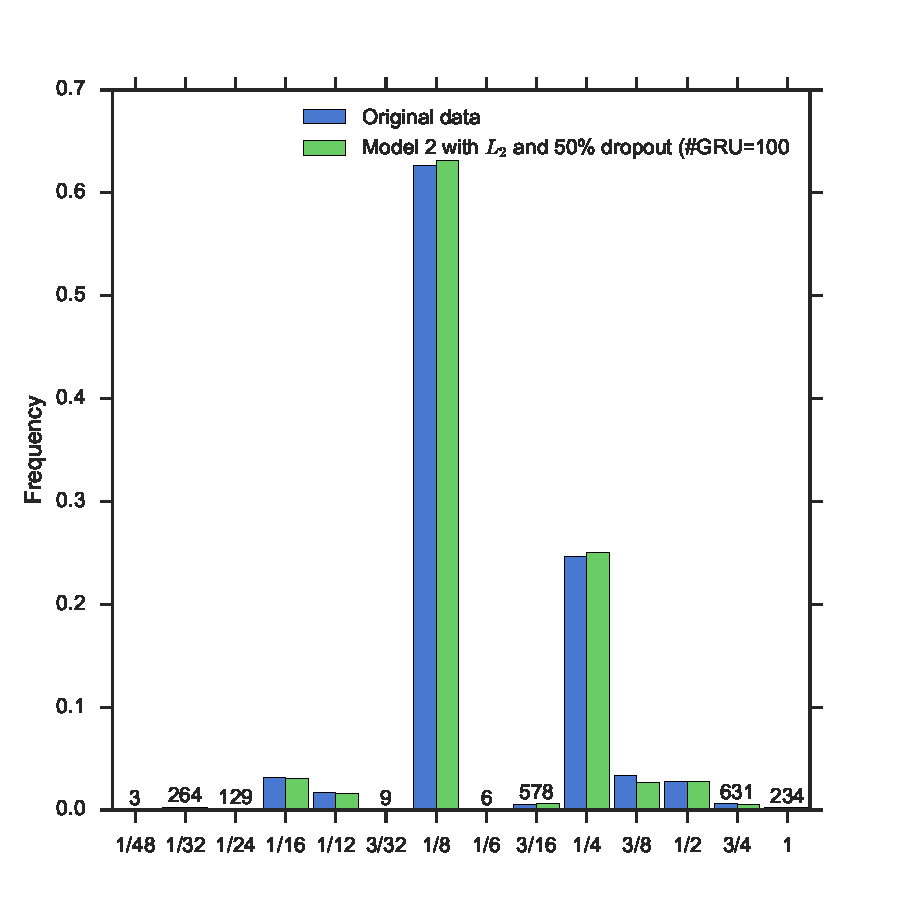
\includegraphics{models_duration_freq_barplot}
    }
	\hspace*{\fill}
    \caption{Histograms showing statistical frequency of pitch \subcaptionref{fig:histogram_models:pitch} and duration \subcaptionref{fig:histogram_models:duration} classes.)
    }
    \label{fig:histogram}
\end{figure*}

% \subsection*{EHR synopsis}

% We expect our model to be able to predict future diagnoses better than baseline methods like logistic regression and the frequency baseline test given in Doctor AI. At the same time, the model will learn to recognise specific patterns in the patient history that will enhance the models predictive power. These patterns can be investigated and used as important markers for doctors to analyse the patient history and whether later complications can be expected and avoided.

% In the worst-case scenario, we are not successful in achieving the above.
